\chapter{Spectral Method}
\label{chap:spectral-method}
In this chapter we will construct a spectral method in the basis of Jacobi polynomials to explore the solution of equilibrium distributions $\hat{\rho}(\hatvec{x})$.
Starting from a many-body system and considering the continuous limit as $N_p \goesto \infty$, in \Cref{chap:particle-interaction-theory} we have already established the governing equation of the particle density distribution $\hat{\rho}(\hatvec{x})$ in such a system.

As mentioned in \Cref{chap:particle-interaction-theory}, the numerical approaches will be carried out on the normalised domain $B_1(\vec{0})$ and we will be looking for $\rho \in \functionspace$, whilst in general we are interested in the $\hat{\rho} \in \functionspacehat$ solving \href{def:the-problem}{our problem}.
Both versions are related by $\hat{\rho}(\hatvec{x}) = \rho(\vec{x})$ and $\hatvec{x} := R \vec{x}$.

Can we put together a numerical method to solve for the equilibrium distribution (cf. \Cref{def:equilibrium-measure})?
Let us consider the problem from the bottom up and start from the solution:
The basic idea behind spectral methods is to assume a solution $\rho(\vec{x})$ of the form
$$\rho(\vec{x}) = \sum_{k=0}^{N-1} \rho_k \varphi_k(\vec{x})\,,\quad \rho_k \in \R, \varphi_k: \R^d \mapsto \R\,,\quad k = 0, ..., N-1\,,$$
with $N$ coefficients $\vec{\rho} := \left(\rho_0, ..., \rho_{N-1}\right)^T$ multiplying $N$ basis functions $\varphi_k$.

\pagebreak
\section{Special Functions}
The following section will introduce a few necessary objects and tools to understand the basis of functions we are working with to construct the spectral method, the basis of Jacobi polynomials.

We start with the Pochhammer symbol, another name for the \textit{rising factorial}, an unusual notation for a function but standard in the context of the special functions that will be introduced on top of it.
\begin{definition}{Rising Factorial (Pochhammer Symbol)}{rising-factorial}
  The $n$th rising factorial of $x \in \R$ is given by
  $$(x)_n := \prod_{k=0}^{n-1} (x+k) \,\in \R\,.$$
\end{definition}

For example, $(3.141)_5 = 3.141 \cdot 4.141 \cdot 5.141 \cdot 6.141 \cdot 7.141$.

\begin{remark}{Nonpositive integer rising factorial}{nonpositive-pochhammer}
  When the argument is a nonpositive integer, the rising factorial
  $(-m)_n = -m \cdot (-m+1) \cdot ... \cdot (-m+n-1)$
  vanishes when $n \ge m+1$ for $n \in \N$ and $m \in \N_0$ as $0$ is among the factors.
\end{remark}


As a second prerequisite, we introduce the closely intertwined beta- and gamma-functions (\Cref{def:beta-function}, \Cref{def:gamma-function}).
\begin{definition}{Gamma Function}{gamma-function}
  Aligning with the factorial for integer arguments, $\Gamma: \R^+ \mapsto \R$ is given by
  $$\Gamma(x) := \int_0^\infty t^{x-1}\e^{-t} \ddt\,.$$
\end{definition}

\begin{definition}{Beta Function}{beta-function}
  $B: \R^+\times\R^+ \to \R$ is given by
  $$B(x_1, x_2) := \int_0^1 t^{x_1-1}(1-t)^{x_2-1} \ddt\,.$$
\end{definition}

Note that following from this definition, there is a relationship with the gamma-function
\begin{equation}
  B(x_1, x_2) = \frac{\Gamma(x_1) \Gamma(x_2)}{\Gamma(x_1 + x_2)}\,.
  \label{eq:beta-gamma}
\end{equation}


Using the Pochhammer symbol introduced in \Cref{def:rising-factorial}, we can now define the generalised hypergeometric series ${}_pF_q$ (cf. \Cref{def:generalised-hypergeometric-series}) and a special case of it, the Gaussian hypergeometric function (cf. \Cref{lemma:gaussian-hypergeometric-function}).
\begin{definition}{Generalised Hypergeometric Series}{generalised-hypergeometric-series}
  The generalised hypergeometric series ${}_pF_q: \R^p \times \R^q \times \C \mapsto \C$ with $p, q \in \N$ is defined by
  $${}_2F_1\left(\begin{matrix}a_{1}, \ldots, a_{p} \\b_{1}, \ldots, b_{q}\end{matrix}; z\right) := \sum _{k=0}^{\infty }{\frac {(a_{1})_{k}\cdots (a_{p})_{k}}{(b_{1})_{k}\cdots (b_{q})_{k}}}\,{\frac {z^{k}}{k!}}\,,$$
  where $(\cdot)_k$ denotes the rising factorial (cf. \Cref{def:rising-factorial}).
\end{definition}

Note that any permutation of the first (``top'') arguments $a_1, ..., a_p$ leaves the function unchanged due to commutativity of multiplication on $\C$. The same holds for the second (``bottom'') arguments $b_1, ..., b_q$.

\begin{lemma}{Gaussian Hypergeometric Function}{gaussian-hypergeometric-function}
  The $p=2$, $q=1$ special case of the generalised hypergeometric series can also be evaluated by
  $${}_2F_1\left(\begin{matrix}a_{1}, -n \\b_{1}\end{matrix}; z\right) = \sum_{k=0}^n (-1)^k \binom{n}{k} \frac{(a_1)_k}{(b_1)_k}z^k\,,$$
  when the second argument $a_2 = -n$ is a nonpositive integer, so $n \in \N_0$.
\end{lemma}
\begin{proof}
  Starting from the definition of the generalised hypergeometric series ${}_pF_q$ with $p=2$ and $q=1$ (\Cref{def:generalised-hypergeometric-series}),
  $${}_2F_1\left(\begin{matrix}a_{1}, -n \\b_{1}\end{matrix}; z\right) = \sum_{k=0}^{\infty} \frac{(a_1)_k (-n)_k}{(b_1)_k} \frac{z^k}{k!} = \sum_{k=0}^{n} \frac{(a_1)_k (-n)_k}{(b_1)_k} \frac{z^k}{k!}\,,$$
  which can be terminated at $k=n$ due to \Cref{remark:nonpositive-pochhammer}, we can express
  $$\frac{(-n)_k}{k!} = \binom{-n+k-1}{k} = (-1)^k \binom{1+n-k+k-1}{k} = (-1)^k \binom{n}{k}$$
  using a well-known relation between the Pochhammer symbol and the binomial coefficient which immediately leads us to  % TODO: where can one find this well-known relation?
  $${}_2F_1\left(\begin{matrix}a_{1}, -n \\b_{1}\end{matrix}; z\right) = \sum_{k=0}^n \binom{n}{k} \frac{(a_1)_k}{(b_1)_k}(-z)^k\,,$$
  concluding the proof.
\end{proof}

Note that these functions are generally tricky to evaluate efficiently, recent advancements have enabled their usage in a broader range of applications \parencite{2008-hypergeometric-functions-jl-1,2017-hypergeometric-functions-jl-2,2023-hypergeometric-functions-jl-3}.
Implementations are available in the \href{https://github.com/JuliaMath/HypergeometricFunctions.jl}{HypergeometricFunctions.jl} package in Julia.

More details on the Gaussian hypergeometric series, sometimes simply referred to as the hypergeometric function, its defining differential equation origin, modular interpretations and symmetries may be found in the 1997 book \citetitle{1997-hypergeometric-functions-my-love} \parencite{1997-hypergeometric-functions-my-love}.


\pagebreak
\section{Orthogonal Polynomials Forming a Basis}
In order to efficiently construct a spectral method, we need an orthogonal basis.
\begin{definition}{Orthogonal Polynomials}{orthogonal-polynomials}
  Are univariate polynomials
  $$p_n: \R \mapsto \R, \; p_n(x) = \sum_{k=0}^{n} c_k x^k\,.$$
  that form an orthogonal basis under some inner product $\langle p_n, p_m \rangle_w$ with weight function $w(x)$, given by
  $$\langle f, g \rangle_w := \int_{-1}^{1} f(x) g(x) w(x) \,\ddx\,.$$
\end{definition}

\begin{remark}{}{symmetry-of-inner-product}
  The inner product satisfies $\langle x\mapsto xf(x), g \rangle_w = \langle f, x \mapsto xg(x)\rangle_w$.
\end{remark}

\begin{theorem}{Three-Term Recurrence Relationship}{three-term-recurrence-relationship}
  All orthogonal polynomials $\{p_0, p_1, p_2, ...\}$ (cf. \Cref{def:orthogonal-polynomials}) have (at least) a three-term recurrence relationship of the form
  $$A_n p_{n+1}(x) = B_n p_n(x) + C_n p_{n-1}(x)\,.$$
\end{theorem}
\begin{proof}
  Consider ``$x p_n$''$:= x \mapsto x p_n(x)$, a polynomial with $\deg(x p_n) \le n+1$.
  By the linear independence of all orthogonal polynomials $p_n$ with respect to the inner product $\langle \cdot, \cdot \rangle_w$, it must be possible to write
  $$x p_n(x) = \sum_{k=0}^{n+1} \hat{a}_k p_k(x)\,,\quad \text{for some}~\hat{a}_k \in \R, k=0, ..., n+1\,.$$
  Now, for all $n \ge 0$ and $m \le n+1$ we have
  $$\langle xp_n, p_m \rangle_w = \sum_{k=0}^{n+1} \hat{a}_k \langle p_k, p_m \rangle_w = \sum_{k=0}^{n+1} \hat{a}_k \delta_{i,k} = \hat{a}_m \langle p_m, p_m \rangle_w\,,$$
  due to the orthogonality relationship (\Cref{thm:jacobi-orthogonality-condition}).
  Therefore,
  \begin{equation}
    \hat{a}_m = \frac{\langle xp_n, p_m \rangle_w}{\langle p_m, p_m \rangle_w} \quad\text{for all}~m \le n+1\,.
    \label{eq:three-term-step}
  \end{equation}

  But when \underline{$m < n-1$}, we have $\deg(xp_m) < n$ so $x p_m(x) = \sum_{k=0}^{n-1} \hat{b}_k p_k(x)$ for some (potentially 0) $\hat{b}_k \in \R$, and therefore $\langle p_n, xp_m \rangle_w = \sum_{k=0}^{n-1} \hat{b}_k \langle p_n, p_k \rangle_w = 0$,
  which, by the symmetry of the inner product (\Cref{remark:symmetry-of-inner-product}), also implies $\langle x p_n, p_m \rangle_w = 0$ which, by \Cref{eq:three-term-step}, allows us to conclude that the earlier coefficients $\hat{a}_m = 0$.

  % And obviously, even if we assumed higher-order coefficients in the expansion of $xp_n$, when $m > n+1 \Leftrightarrow n < m-1$, $\deg(xp_n) < m$ and so all later coefficients $\hat{a}_m = 0$.

  We recall that $xp_n(x) = \sum_{k=0}^{n+1} \hat{a}_k p_k(x)$, which in combination with our insights on the $\hat{a}_m$ above means that
  $$xp_n(x) = \hat{a}_{n-1} p_{n-1}(x) + \hat{a}_{n} p_n(x) + \hat{a}_{n+1} p_{n+1}(x)\,,$$
  concluding the proof.
\end{proof}

For example, for the Chebyshev polynomials (cf. \Cref{def:chebyshev-polynomials}) we have
$$T_{k+1}(x) = 2x T_k(x) - T_{k-1}(x) \,.$$

% From HeatFun:
% \begin{theorem}{Chebyshev recursion formula}{chebrecursion}
%   The \chebyshev polyomials satisfy the three-term recurrence relation $$T_{k+1}(x) = 2x T_k(x) - T_{k-1}(x) \,.$$
% \end{theorem}
% \begin{proof}{\parencite{atap}.}
%   For $k > 1$, we have
%   \begin{align*}
%     2x T_k(x) - T_{k-1}(x) & = 2x \cdot \frac{1}{2} (z^k + z^{-k}) - \frac{1}{2} (z^{k-1} + z^{-(k-1)})                     \\
%                            & = 2 \frac{1}{2}(z + z^{-1}) \cdot \frac{1}{2}(z^k + z^{-k}) - \frac{1}{2} (z^{k-1} + z^{-k+1}) \\
%                            & = \frac{1}{2} (z^{k+1} + z^{k-1} + z^{-k+1} + z^{-k-1}) - \frac{1}{2} (z^{k-1} + z^{-k+1})     \\
%                            & = \frac{1}{2} (z^{k+1} + z^{-(k+1)}) = T_{k+1}(x)
%   \end{align*}
% \end{proof}


The Jacobi polynomials are then defined from ${}_2F_1$ as follows:
\begin{definition}{Jacobi Polynomials}{jacobi-polynomials}
  Let $P^{(a, b)}: \C \mapsto \C$ with
  $$P^{(a,b)}_n(x) = {\frac{(a +1)_{n}}{n!}}\,{}_{2}F_{1}\left(-n,1+a +b +n;a +1;{\tfrac  {1}{2}}(1-x)\right)$$
  So are defined using the Gaussian Hypergeometric Function (cf. \Cref{def:gaussian-hypergeometric-function}) and the Pochhammer symbol.
  Which is equivalent to
  $$P_{n}^{{(a, b)}}(x)={\frac  {\Gamma (a +n+1)}{n!\,\Gamma (a +b +n+1)}}\sum _{{m=0}}^{n}\binom{n}{m}{\frac{\Gamma (a +b +n+m+1)}{\Gamma (a +m+1)}}\left({\frac{x-1}{2}}\right)^{m}\,.$$
  where $\Gamma (x)=\int _{0}^{\infty }t^{x-1}e^{-t}\,\ddt$ (with $\Re(x)>0$) is the gamma function \footnote{Recall that for integer arguments $k \in \N$, it equals the factorial of $(k-1)$ so $\Gamma(k) = (k-1)!$.}.

  Gegenbauer Polynomials (cf. \Cref{def:gegenbauer-polynomials}) are a special case. And
  Chebyshev Polynomials (cf. \Cref{def:chebyshev-polynomials}) are a special case of them.
\end{definition}

Following from this definition,
\begin{align*}
  P_0^{(a, b)}(x)   & = 1                            \\
  P_{1}^{(a, b)}(x) & = (a+1)+(a+b+2){\frac{x-1}{2}}
\end{align*}
and so on. Note that obviously, $\deg\left(P_k^{(a, b)}\right) = k$.

Nice Spectral Properties:
\begin{itemize}
  \item Differentiation
  \item Three-Term Recurrence
  \item why are they better than just Chebyshev?
\end{itemize}

Note that in this manuscript we will use the dot-product notation
$$f(x) = \sum_{k=0}^{N-1} f_k P_k^{(a, b)}(x) \qLRq f(x) = \vec{f} \cdot \vec{P}^{(a, b)}(x)\,,$$
to express that a function $f$ is a linear combination of basis polynomials with coefficients $\vec{f} = (f_0, ..., f_{N-1})^T \in \R^N$.
So $\vec{P}^{(a, b)}(x) \in \R^N$ is the vector of Jacobi polynomials $P^{(a, b)}_0(x)$, $P^{(a, b)}_1(x)$, ..., $P^{(a, b)}_{N-1}(x)$.

Jacobi polynomials $P_n^{(a,b)}(x)$ are orthogonal on $[-1,1]$ w.r.t. the weight function
\begin{equation*}
  w^{(a,b)}(x)=(1-x)^a (1+x)^b\,,
\end{equation*}
so they satisfy
\begin{align*}\label{eq:orthogonalityconditionJacobi}
  \int_{-1}^1(1-x)^a(1+x)^bP_n^{(a,b)}P_m^{(a,b)}\,\ddx = \frac{2^{a+b+1} \Gamma (a+n+1) \Gamma (b+n+1)}{n! (a+b+2 n+1) \Gamma (a+b+n+1)} \delta_{n,m}\,,
\end{align*}
with $a	,b>-1$, which uniquely determines $P_n^{(a,b)}(x)$. The special case of $a=b$ corresponds to the ultraspherical or Gegenbauer polynomials, while the case $a=b=0$ corresponds to the Legendre polynomials \cite{2018-nist}.

\begin{itemize}
  \item This basis yields a \textbf{sparse}, and in particular, \textbf{banded} operator.
\end{itemize}

\begin{figure}[H]
  \centering
  \label{fig:jacobi-expansions-error}
  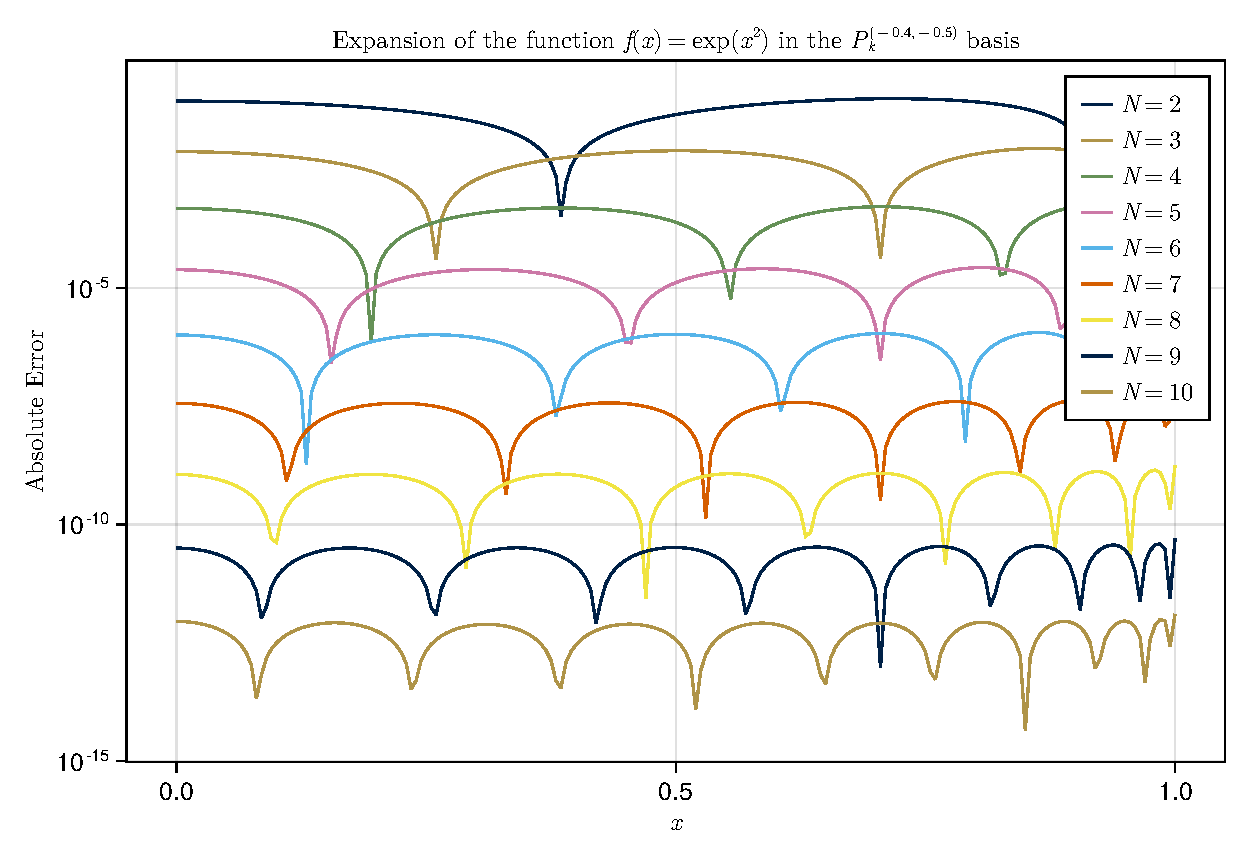
\includegraphics[width=0.7\linewidth]{results/jacobi-expansions.pdf}
  \caption[Convergence of Jacobi basis expansion]{Convergence of the Jacobi polynomial expansion $f_N(x) = \sum_{k=0}^{N-1} P_k^{(a, b)}(x)$ of an example function $f(x) = \e^{x^2}$ with $a = -\frac{3}{4}$ and $b = -\frac{1}{2}$. Each added term improves the absolute error between the function and its expansion by a factor, so we have exponential convergence. The number of ``arches'' of each solution error function, occuring from the roots of $f(x) - f_N(x)$, approximately equals the order $N$.}
\end{figure}

% TODO: Convergence speed according to theory is...?

% \begin{definition}{Gegenbauer Polynomials}{gegenbauer-polynomials}
  \begin{center}\rule{0.5\linewidth}{0.5pt}\end{center}

  \hypertarget{alias-ultraspherical-polynomials}{%
    \subsection{alias: Ultraspherical
      Polynomials}\label{alias-ultraspherical-polynomials}}

  Are a special case of the Jacobi Polynomials (cf. \Cref{def:jacobi-polynomials}) and form an
  Orthonormal Basis (cf. \Cref{def:orthonormal-basis}) under the weight given by
  \[w(x)=(1+x)^\alpha\]
\end{definition}

% \begin{definition}{Chebyshev Polynomials}{chebyshev-polynomials}
  Of the first kind: \[T_k(x)\] Of the second kind: \[U_k(x)\] Also have a
  {[}{[}Three-Term Recurrence Relationship{]}{]}.
\end{definition}

\begin{remark}{}{jacobi-matrix}
  The Jacobi operator is the matrix \(X \in \R^{N \times N}\) satisfying
  $$x \cdot \vec{P}^{(a,b)}(x) = \vec{P}^{(a,b)}(x) \cdot X^T\,.$$
\end{remark}

The terms in the Jacobi operator are closely connected to the three-term recurrence relationship (cf. \Cref{thm:three-term-recurrence-relationship}), even making the matrix tridiagonal.


% \pagebreak
\section{Working Towards a Solution}
Finally, now that we have established the basis functions, we can write down an ansatz $\rho: B_1(\vec{0}) \mapsto \R$ for the solution of \hyperref[def:the-problem]{the problem}, of the form
\begin{equation}
  \rho[\vec{\rho}](\vec{x}) = \rho(\vec{x}) := \left(1-\norm{\vec{x}}^{2}\right)^{m - \frac{\alpha + d}{2}} \sum_{k=0}^{N-1} \rho_k P_{k}^{\left(m - \frac{\alpha + d}{2},\frac{d-2}{2}\right)}(2 \norm{\vec{x}}^{2}-1)\,.
  \label{eq:ansatz}
\end{equation}
with $P_k^{(a, b)}$ the Jacobi polynomials and $\{\rho_k\}_{k=0, ..., N-1}$ the coefficients.
% TODO: is it alpha or beta in the exponent of (1-y\^{}2)?

The spectral method can then be written as a linear system of the coefficients $\vec{\rho}$ as we will see in the next section.
In order to establish said linear system, we first need to introduce the \textit{inverse fractional Laplacian}, helping us with the evaluation of the power law potential integral involving radial Jacobi polynomials given in \Cref{thm:theorem216}, the most important result of this chapter.

Let $(-\Delta)^{-\gamma}$ denote the inverse fractional Laplacian $\Delta := \nabla^2$ with power $\gamma \in (0, 1)$.
There are numerous equivalent definitions available (cf. \cite{2015-fractional-laplacian-definitions}), within the context of potential theory the Riesz potential definition (\Cref{def:riesz-potential}) is the most common.

% TODO: can we accept any gamma?
\begin{definition}{Riesz Potential}{riesz-potential}
  For a given function $u: \R^d \mapsto \R$ and $\gamma \in \R$, its \textit{Riesz potential} $I_{\gamma}[u]$ is given by
  $$I_{\gamma}[u](\vec{x}) := \frac{2^{-\gamma} \Gamma(\tfrac{d-\gamma}{2})}{\pi^{d/2} \Gamma(\gamma/2)} \int_{\R^d} \frac{u(\vec{z})}{\norm{\vec{x}-\vec{z}}^{d-\gamma}} \dd\vec{z}\,.$$
\end{definition}

For $\gamma \in (0, d)$, the Riesz potential is equivalent to the inverse fractional Laplacian, so $(-\Delta)^{-\gamma} = I_\gamma$.
So in the case of positive power law kernels, the equivalence to the inverse fractional Laplacian does not apply.
Results on the integral will hold nevertheless and we move on to stating \Cref{thm:theorem216} from \cite{2021-arbitrary-dimensions} verbatim.

\begin{theorem}{Power Law Potential of the $n$th Jacobi Polynomial}{theorem216}
  On the $d$-dimensional unit ball $B_1(\vec{0})$ the power law potential, with power $\alpha \in(-d,2+2m-d)$, $m\in\mathbb{N}_0$ and $\beta>-d$, of the $n$th weighted radial Jacobi polynomial $(1-\norm{\vec{y}}^2)^{m-\frac{\alpha+d}{2}}P_n^{\left(m-\frac{\alpha+d}{2},\frac{d-2}{2}\right)}\left(\jacobiarg{y}\right)$ reduces to a Gaussian hypergeometric function as follows:
  \begin{align*}
    I_{m,n}^{\alpha,\beta}(\vec{x}) & = \int_{B_1(\vec{0})} \norm{\vec{x}-\vec{y}}^\beta \left(1-\norm{\vec{y}}^2\right)^{m-\frac{\alpha+d}{2}} P_{n}^{\left(m-\frac{\alpha+d}{2},\frac{d-2}{2}\right)}\left(\jacobiarg{y}\right) \dd\vec{y}                                                                                                                                                                                                             \\
                                    & = \tfrac{\pi ^{d/2} \Gamma \left(1+\frac{\beta}{2}\right) \Gamma \left(\frac{\beta+d}{2}\right) \Gamma \left(m+n-\frac{\alpha+d}{2}+1\right)}{\Gamma \left(\frac{d}{2}\right) \Gamma (n+1) \Gamma \left(\frac{\beta}{2}-n+1\right) \Gamma \left(\frac{\beta-\alpha}{2}+m+n+1\right)}{}_2F_1\left(\begin{matrix}n-\frac{\beta}{2}, -m-n+\frac{\alpha-\beta}{2} \\\frac{d}{2}\end{matrix};\norm{\vec{x}}^2\right)\,.
  \end{align*}
\end{theorem}

\begin{proof}[Proof (adapted from \cite{2021-arbitrary-dimensions}, Section 2.5)]
  ~\\
  We begin by applying \Cref{lemma:jacobi-polynomial-series} to the inside of the integrand.
  \begin{align*}
    I := \int_{B_1(\vec{0})} & \norm{\vec{x}-\vec{y}}^\beta \weight{y} \jacobi[n]{y} \dd\vec{y}                                                                                             \\
                             & = C_{a,b,n} \sum_{k=0}^n \binom{n}{k} C_{a,b,n,k} \int_{B_1(\vec{0})} \norm{\vec{x}-\vec{y}}^\beta \weight{y} \left(\norm{\vec{y}}^2 - 1\right)^k \dd\vec{y} \\
                             & = C_{a,b,n} \sum_{k=0}^n \binom{n}{k} C_{a,b,n,k} (-1)^k \int_{B_1(\vec{0})} \norm{\vec{x}-\vec{y}}^\beta \weight[a+k]{y} \dd\vec{y}
  \end{align*}
  where $a := m-\frac{\alpha+d}{2}$ and $b := \frac{d-2}{2}$.
  Note that from the first to the second line, we used $\frac{z-1}{2} = \frac{2\norm{\vec{y}}^2-1 - 1}{2} = \norm{\vec{y}}^2 - 1$.

  The constants are
  \begin{align*}
    C_{a,b,n}   & := \frac{\Gamma(a+1+n)}{n! \Gamma(1+a+b+n)}     \\
    C_{a,b,n,k} & := \frac{\Gamma(1+a+b+n + k)}{\Gamma(a+1+k)}\,.
  \end{align*}

  We identify the remaining integral as the Riesz potential $I_{\beta+d}[u](\vec{x})$, cf. \Cref{def:riesz-potential}, of the function $u(\vec{y}) := \left(1-\norm{\vec{y}}^2\right)^{a+k}$, which we can evaluate using Lemma 2.4 from \cite{2011-porous-medium-1}:
  \begin{align*}
    \int_{B_1(\vec{0})} & \norm{\vec{x}-\vec{y}}^\beta \weight[a+k]{y} \dd\vec{y} = c_{\beta+d} I_{\beta+d}\left[\vec{y} \mapsto \left(1-\norm{\vec{y}}^2\right)^{a+k}\right](\vec{x}) \\
                        & = c_{\beta+d} C_{a+k, \beta, d} \cdot {}_2F_1\left(\begin{matrix}\frac{d-(\beta+d)}{2}, -a-k-\frac{\beta+d}{2} \\d/2\end{matrix}; \norm{\vec{x}}^2\right)    \\
                        & = c_{\beta+d} C_{a+k, \beta, d} \cdot {}_2F_1\left(\begin{matrix}-\beta/2, -m-k+\frac{\alpha-\beta}{2} \\d/2\end{matrix}; \norm{\vec{x}}^2\right)\,,
  \end{align*}
  as $-a-k-\frac{\beta+d}{2} = -m + \frac{\alpha+d}{2} -k - \frac{\beta+d}{2} = -m-k+\frac{\alpha-\beta}{2}$ with constants
  \begin{align*}
    c_{\beta+d}       & := \frac{2^{\beta+d} \pi^{d/2} \Gamma\left(\frac{\beta+d}{2}\right)}{\Gamma(-\beta/2)}                      \quad \text{\textcolor{gray}{from aforementioned definition of the Riesz potential}} \\
    C_{a+k, \beta, d} & := \frac{\Gamma(a+k+1) \Gamma(-\beta/2)}{2^{\beta+d}\Gamma(d/2) \Gamma\left(a+k+\frac{\beta+d}{2}+1\right)} \quad \text{\textcolor{gray}{from Lemma 2.4}}\,,
  \end{align*}
  and therefore
  $$c_{\beta+d} C_{a+k, \beta, d} = \frac{\cancel{2^{\beta+d}} \pi^{d/2} \Gamma\left(\frac{\beta+d}{2}\right) \Gamma(a+k+1) \cancel{\Gamma(-\beta/2)}}{\cancel{\Gamma(-\beta/2)} \cancel{2^{\beta+d}}\Gamma(d/2) \Gamma\left(a+k+\frac{\beta+d}{2}+1\right)} = \frac{\pi^{d/2}B\left(\tfrac{\beta+d}{2}, a+k+1\right)}{\Gamma(d/2)}\,,$$
  using \Cref{eq:beta-gamma}.
  So that finally,
  \begin{align*}
    \int_{B_1(\vec{0})} & \norm{\vec{x}-\vec{y}}^\beta \weight[a+k]{y} \dd\vec{y}                                                                                                                                                         \\
                        & =\frac{\pi^{d/2}}{\Gamma(d/2)} B\left(\tfrac{\beta+d}{2}, m-\tfrac{\alpha+d}{2}+k+1\right) \cdot {}_2F_1\left(\begin{matrix}-\beta/2, -m-k+\frac{\alpha-\beta}{2} \\d/2\end{matrix}; \norm{\vec{x}}^2\right)\,.
  \end{align*}

  Plugging this back into the original form above, carrying along the same parameters,
  \begin{align*}
    I = C_{a,b,n} \sum_{k=0}^n \binom{n}{k} C_{a,b,n,k} (-1)^k \frac{\pi^{d/2}}{\Gamma(d/2)} B\left(\cdot, \cdot\right) {}_2F_1\left(\dots; \norm{\vec{x}}^2\right)\,
  \end{align*}
  we can apply Equation (2.1) in \cite{2021-arbitrary-dimensions} after some algebra, the special case of an identity given in \cite{1986-crazy-hypergeometric-properties} to obtain a ${}_3F_2$ (three terms in the numerator, two in the denominator) function
  \begin{align*}
    I \propto {}_3F_2\left(\begin{matrix}-\beta/2, n-\beta/2, -m-n+\frac{\alpha-\beta}{2} \\d/2, -\beta/2\end{matrix}; \norm{\vec{x}}^2\right)\,,
  \end{align*}
  which we expand into its \Cref{def:generalised-hypergeometric-series} to see that two terms cancel:
  \begin{align*}
    I \propto \sum_{k=0}^{\infty} \frac{\cancel{(-\beta/2)_k}, (n-\beta/2)_k, \left(-m-n+\frac{\alpha-\beta}{2}\right)_k}{(d/2)_k \cancel{(-\beta/2)_k}} \frac{\norm{\vec{x}}^{2k}}{k!}\,,
  \end{align*}
  which results back in a ${}_2F_1$ function (two terms in the numerator, one in the denominator), the so-called Gaussian hypergeometric function, cf. \Cref{lemma:gaussian-hypergeometric-function}, and after combining $C_{a,b,n}$, $C_{a,b,n,k}$, $\frac{\pi^{d/2}}{\Gamma(d/2)}$ with the gamma-function expansion of $B\left(\tfrac{\beta+d}{2}, m-\tfrac{\alpha+d}{2}+k+1\right)$ according to \Cref{eq:beta-gamma}, and cancelling terms, one finally obtains
  $$I = \tfrac{\pi^{d/2} \Gamma \left(1+\frac{\beta}{2}\right) \Gamma \left(\frac{\beta+d}{2}\right) \Gamma \left(m+n-\frac{\alpha+d}{2}+1\right)}{\Gamma \left(\frac{d}{2}\right) \Gamma (n+1) \Gamma \left(\frac{\beta}{2}-n+1\right) \Gamma \left(\frac{\beta-\alpha}{2}+m+n+1\right)}{}_2F_1\left(\begin{matrix}n-\frac{\beta}{2}, -m-n+\frac{\alpha-\beta}{2} \\\frac{d}{2}\end{matrix};\norm{\vec{x}}^2\right)\,,$$
  concluding the proof.
\end{proof}

Lemma 2.4 from \cite{2011-porous-medium-1,1967-formulas-and-theorems} is based on the \textit{Weber-Schafheitlin} integral of two Bessel functions given in \cite{1945-bessel-integral}.
The Weber-Schafheitlin integrals are related to the fractional Laplacians of aforementioned functions because the Fourier transform of ${}_2F_1$ is a Bessel function.
For a more generalised version of Lemma 2.4, see \cite{2014-barenblatt}.

Also note that for even integer $\beta$, the prefactor in \Cref{thm:theorem216} sometimes contains an expression of the form $\Gamma(-n),\, n \in \N$ which in principle leads to undefined behaviour (cf. \Cref{def:gamma-function} together with the property that $k \Gamma(k) = \Gamma(k+1)$).
However, one can consider the limit as $x \in \R^+$ approaches an integer $n$ to find that
$$\lim_{x \goesto n} \Gamma(-x) = (-1)^{n-1} \infty\,, \quad\text{or equivalently}\quad \lim_{x \goesto n} \frac{1}{\Gamma(-x)} = 0\,,$$
in which case we are lucky because $\Gamma(\beta/2-n+1)$ appears in the denominator of the prefactor and without any singularities in the numerator we can safely evaluate the entire expression to $0$.

Because $I_{m,n}^{\alpha,\beta}(\vec{x})$ only depends on the squared radius $r^2 = \norm{\vec{x}}^2$, let it also be denoted by $I_{m,n}^{\alpha,\beta}(r^2) = I_{m,n}^{\alpha,\beta}(\vec{x})$.
Further, let
\begin{equation}
  \bar{I}_{m,n}^{\alpha,\beta} := \frac{\left\langle x \mapsto I\left(\frac{x+1}{2}\right), P_0^{(a, b)} \right\rangle}{\left\langle P_0^{(a, b)}, P_0^{(a, b)} \right\rangle} = \frac{1}{h_0^{(a, b)}} \int_{-1}^{1} I_{m,n}^{\alpha,\beta}\left(\frac{x+1}{2}\right) w^{(a,b)}(x) \,\ddx\,,
  \label{eq:0th-coeff-of-I}
\end{equation}
denote the 0th coefficient in a Jacobi expansion of $I_{m,n}^{\alpha,\beta}(\vec{x})$ (recall that $r^2 = \frac{x+1}{2}$ and $P_0^{(a, b)}(x) = 1$) with $h_k := \left\langle P_k^{(a, b)}, P_k^{(a, b)} \right\rangle$ the normalisation coefficients of the basis.


% \Cref{thm:theorem216} gives an explicit expression for the main integral \(\mathcal{Q}^{\beta}: L \mapsto L\), an operator from the function space \(L\) to the function space \(L\), we are interested in:
% which is used to construct the spectral method operator \(Q^\beta\) (cf. \Cref{def:power-law-operator}), acting on the coefficients \(\vec{\rho}\).

Adding to our collection of tools, in order to solve the problem given in \Cref{def:the-problem} we need to normalise the solution by its mass.
The normalisation constant is given in \Cref{lemma:mass}, based only on a single coefficient $\rho_0$, allowing for a highly efficient renormalisation.
\begin{lemma}{Mass of the Solution}{mass}
  For a given solution $\rho: B_1(\vec{0}) \mapsto \R$, its \textit{mass} $M \in \R$ is given by \Cref{eq:measure-mass}.
  Provided the appropriate ansatz given in \Cref{eq:ansatz}, an expansion of weighted radial Jacobi polynomials with coefficients $\rho_k$, its \textit{mass} is given by
  \begin{align*}
    M := \int_{\supp(\rho)} \rho(y) \,\ddy = \frac{\pi^{{d/2}}\Gamma (a+1)}{\Gamma \left(a+{d/2}+1\right)}\, \rho_0\,,
  \end{align*}
  so solely depending on the first coefficient $\rho_0$.
\end{lemma}
\begin{proof}[Proof (adapted from \cite{2021-arbitrary-dimensions})]
  To shorten notation, let $b := \frac{d-2}{2}$.
  The domain and radial symmetry of our problem suggests the use of hyperspherical coordinates:
  \begin{align*}
    M = \int_{B_1(\vec{0})} \rho(\vec{x}) \,\dd\vec{x} & = \sum_{k=0}^{N-1} \rho_k \int_{B_1(\vec{0})} \weight{x} P_k^{(a,b)}(\jacobiarg{x}) \,\dd\vec{x}                          \\
                                                       & =\sum_{k=0}^{N-1} \rho_k \int_{\partial B_1(\vec{0})} \dd\Omega \int_{r=0}^1 (1-r^2)^a P_k^{(a,b)}(2r^2-1) r^{d-1} \,\ddr \\
                                                       & = \Omega_d \sum_{k=0}^{N-1} \rho_k \int_{r=0}^1 (1-r^2)^a P_k^{(a,b)}(2r^2-1) r^{d-1} \,\ddr\,,
  \end{align*}
  where $\Omega_d = {2\pi^{d/2}} / {\Gamma({d/2})}$ is the surface area of the $d$-dimensional hypersphere (cf. \Cref{lemma:surface-area}) with radius $R = 1$.
  % Note that working with a finite expansion ($N < \infty$), we automatically have
  % $$\int_{B_1} \sum_{k=0}^{N-1} |\rho_k (1-|y|^2)^a P_k^{(a,b)}(2|y|^2-1)| \,\ddy < \infty\,,$$
  % so the exchange of integration and infinite sum in the first line is justified by the Fubini-Tonelli theorem.
  Substituting $u := 2r^2-1$, therefore $r^2 = \frac{1+u}{2}$ and $(1-r^2)^a = \left(\frac{1-u}{2}\right)^a = 2^{-a} (1-u)^a$ as well as $\ddr = \frac{\ddu}{4r}$,
  \begin{align*}
    M & = 2^{-a} \Omega_d \sum_{k=0}^{N-1} \rho_k \int_{u=-1}^1 (1-u)^a P_k^{(a,b)}(u) r^{d-1} \,\frac{\ddu}{4r} \\
      & = 2^{-2} 2^{-a} \Omega_d \sum_{k=0}^{N-1} \rho_k \int_{-1}^1 (1-u)^a P_k^{(a,b)}(u) r^{d-2}\,\ddu\,,
  \end{align*}
  we notice that $r^{d-2} = \left(\frac{1+u}{2}\right)^{\frac{d-2}{2}} = 2^{-b} (1+u)^b$ and so we have
  \begin{align*}
    M & = 2^{-2} 2^{-a} 2^{-b} \Omega_d \sum_{k=0}^{N-1} \rho_k \int_{-1}^1 (1-u)^a (1+u)^{b} P_k^{(a,b)}(u) \,\ddu                                                 \\
      & = 2^{-(2+a+b)} \Omega_d \sum_{k=0}^{N-1} \rho_k \int_{-1}^1 (1-u)^a (1+u)^{b} P_k^{(a,b)}(u) P_0^{(a, b)}(u) \,\ddu                                         \\
      & = 2^{1-(2+a+b)} \frac{\pi^{d/2}}{\Gamma(d/2)} \sum_{k=0}^{N-1} \rho_k \, \frac{2^{a+b+1} \Gamma (a+1) \Gamma (b+1)}{0! (a+b+1) \Gamma (a+b+1)} \delta_{0,k} \\
      & = \frac{\pi^{{d/2}}\Gamma (a+1)}{\Gamma \left(a+{d/2}+1\right)} \,\rho_0\,,
  \end{align*}
  which relies on the classical orthogonality condition of the Jacobi polynomials given in \Cref{thm:jacobi-orthogonality-condition} with the $0$th polynomial $P_0(u) = 1$.
\end{proof}

\begin{lemma}{Surface area of the hypersphere}{surface-area}
  The surface area of the d-dimensional hypersphere $\partial B_R(\vec{0})$ is given by
  $$\Omega_{d}(R) = \frac{\dd}{\dd R} V_d(R) = \frac{\dd}{\dd R} \left(\frac{2 \pi^{d/2}}{d \Gamma(d/2)} R^d\right) = \frac{2\pi^{d/2}}{\Gamma({d/2})} R^{d-1}\,.$$
\end{lemma}
\begin{proof}
  We find $\Omega_d$ by evaluation of the $d$-dimensional Gaussian integral
  $$I_d := \int_{\R^d} \e^{-\norm{\vec{x}}^2}\,\dd\vec{x} = \int_{\R} \ddx_1 ... \int_{\R} \ddx_d\, \e^{-x_1^2-...-x_d^2} = \left(\int_{\R} \e^{-x_1^2} \,\ddx_1\right)^d = (I_1)^d\,,$$
  using Fubini's theorem ($I_d < \infty$).
  Considering the case $d = 2$, we have
  $$I_2 = \int_{\R^2} \e^{-\norm{\vec{x}}^2} \,\dd\vec{x} = \int_0^{2\pi} \dd\theta \int_0^\infty r \e^{-r^2} \,\ddr = -2\pi \int_{0}^{-\infty} \e^u \,\frac{\ddu}{2} = \pi \int_{-\infty}^0 \e^u \,\ddu = \pi\,,$$
  taking the classical approach of transitioning to polar coordinates $r, \theta$ (with Jacobi determinant $r^{d-1}$ in the $d$-dimensional case) immediately leading us to $I_1 = \sqrt{\pi}$. Generalising this to higher dimensions $d$ with hyperspherical coordinates,
  $$I_d = \int_{\R^d} \e^{-\norm{\vec{x}}^2} \,\dd\vec{x} = \Omega_d \int_0^\infty r^{d-1} \e^{-r^2}\,\ddr = \Omega_d \int_0^\infty s^{{d/2}-1} \e^{-s} \frac{\dds}{2} = \frac{\Omega_d}{2} \Gamma(d/2)\,,$$
  where once again $r := \norm{\vec{x}}$ and using a substitution $s := r^2$, we must find equality with the above result $I_d = \pi^{d/2}$,
  $$I_d = \pi^{d/2} \overset{!}{=} \frac{1}{2}\Omega_d \Gamma(d/2) \qLRq \Omega_d = \frac{2\pi^{d/2}}{\Gamma(d/2)}\,.$$
  Now integrating over the $R$-ball $B_R(\vec{0})$, we obtain $V_d(R) := |B_R(\vec{0})| = \Omega_d \int_0^R r^{d-1} \,\ddr = \frac{\R^d \Omega_d}{d}$ and therefore $\Omega_{d}(R) = \frac{\dd V_d(R)}{\dd R} = \frac{2 \pi^{d/2}}{\Gamma(d/2)}R^{d-1}$.
\end{proof}


\pagebreak
\section{Derivation of the Operator}
\begin{definition}{Operator}{operator}
  Either the attractive or the repulsive operator can be sparse.

  Obtained using {[}{[}Theorem 2.16{]}{]}. Derivation of the exact
  row/column form on paper ( \#include in My Dissertation (cf. \Cref{def:my-dissertation}))

  \begin{itemize}
    \tightlist
    \item
          {[} {]} What does the solver look like for other kernels?
  \end{itemize}
\end{definition}

Based on the {[}{[}Three-Term Recurrence Relationship{]}{]}.

One can even determine an explicit relationship between the coefficients
in the Jacobi expansion by considering the {[}{[}Jacobi Matrix{]}{]}.

Considering the operator $\hat{Q}^\beta[\rho]$ as in \Cref{thm:theorem216}, from the [[Ansatz]] $\rho(x)$ we have
$$\hat{Q}^{\beta}(x) = \sum_{k=1}^{N} \rho_{k} \int \norm{x-y}^{\beta}(1-\norm{y}^2)^{a}P_{k}^{(a, b)}(2\norm{y}^{2}- 1) \,\ddy$$

For the attractive-repulsive interaction potential $K_{\alpha,\beta}(r)$, the full operator is given by
\begin{align*}
  \mathcal{Q}_{\alpha, \beta}[\hat{\rho}](\hatvec{x}) & := \int_{B_R(\vec{0})} K_{\alpha,\beta}\left(\norm{\hatvec{x} - \hatvec{y}}\right) \hat{\rho}(\hatvec{y}) \,\dd\hatvec{y}                                                               \\
                                                      & = \int_{B_R(\vec{0})} \left(\frac{\norm{\hatvec{x} - \hatvec{y}}^\alpha}{\alpha} - \frac{\norm{\hatvec{x} - \hatvec{y}}^\beta}{\beta}\right) \hat{\rho}(\hatvec{y}) \,\dd\hatvec{y}     \\
                                                      & = \int_{B_1(\vec{0})} \left(\frac{R^\alpha \norm{\vec{x} - \vec{y}}^\alpha}{\alpha} - \frac{R^\beta \norm{\vec{x} - \vec{y}}^\beta}{\beta}\right) \hat{\rho}(R\vec{y}) \, R^d\dd\vec{y} \\
                                                      & = R^d\int_{B_1(\vec{0})} \left(\frac{R^\alpha}{\alpha}\norm{\vec{x} - \vec{y}}^\alpha - \frac{R^\beta}{\beta} \norm{\vec{x} - \vec{y}}^\beta\right) \rho(\vec{y}) \,\dd\vec{y}          \\
                                                      & = \frac{R^{\alpha+d}}{\alpha} \mathcal{Q}^\alpha[\rho](\vec{x}) - \frac{R^{\beta+d}}{\beta} \mathcal{Q}^\beta[\rho](\vec{x})\,,
\end{align*}
where one needs to carefully handle the variable transform with $\dd\hatvec{y} = R^d \dd\vec{y}$ in $d$ dimensions whereas the vectors themselves obey $\hatvec{y} = R \vec{y}$ as established previously.
In matrix form that is,
\begin{equation}
  Q_{\alpha, \beta} := \frac{R^{\alpha+d}}{\alpha} Q^\alpha - \frac{R^{\beta+d}}{\beta} Q^\beta\,,
  \label{eq:full-attrep-operator}
\end{equation}
for some interval radius $R \in \R^+$, usually chosen as the smallest possible $R$ such that $\supp(\rho) \subseteq [-R, R]$.

\begin{figure}[H]
  \centering
  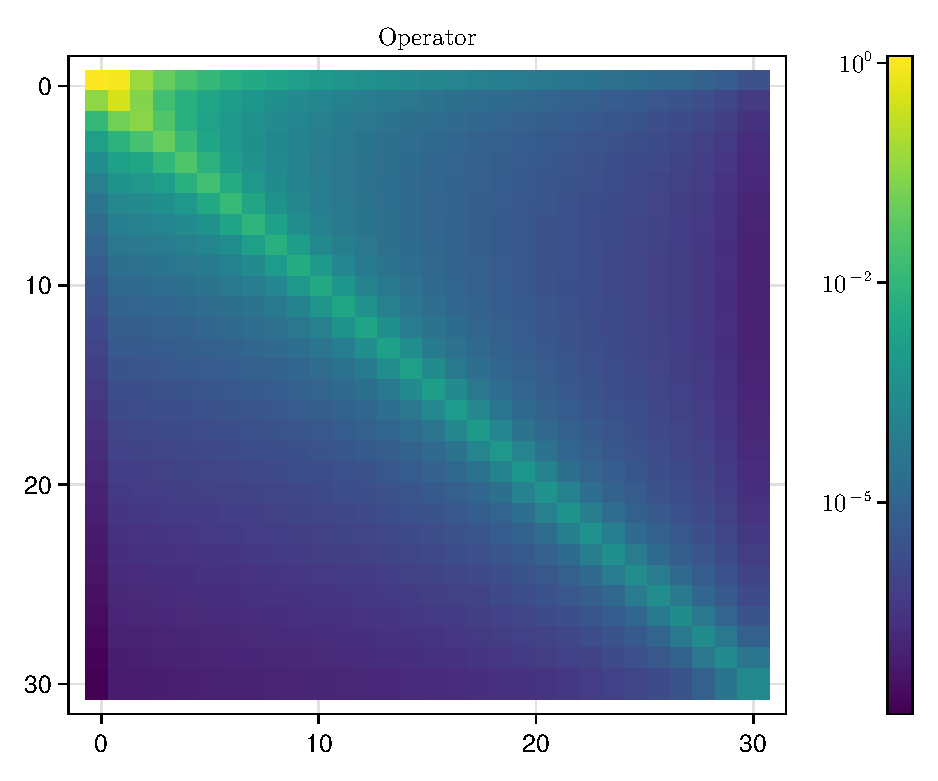
\includegraphics[width=0.5\linewidth]{results/attrep/full-operator.pdf}
  \caption[Combination of the attractive-repulsive operators]{Spy plot of $Q_{\alpha, \beta}$, the combination of the attractive-repulsive operators. Inverting this operator and applying it to $(1, 0, ..., 0)^T \in \R^N$ will yield the unnormalised coefficients $\rho_k$ of the solution expansion given in \Cref{eq:ansatz}.}
  \label{fig:attrep-operator}
\end{figure}


\pagebreak
% Full Section:
\section{Solving a Linear System}
Once the operator is computed, we are now looking for a set of solution coefficients $\vec{\rho} \in \R^N$ such that the total energy $E = E_{\rm kin} + U = U = U_K[\hat{\rho}]$ (in the presence of friction, the kinetic energy will eventually dissipate, cf. \Cref{chap:particle-interaction-theory}) on the domain $D = B_R(\vec{0})$ is constant.
That means, we are looking for $\vec{\rho} \in \R^N$ such that
\begin{equation}
  \mathcal{Q}[\rho](\vec{x}) = \tilde{E}(\vec{x}) = E\,,
\end{equation}
where we can expand $\tilde{E}(\vec{x}) = \jacobivec{x} \cdot \vec{E}$ into Jacobi polynomials with coefficients $\vec{E} = E \vec{e_1} = (E, 0, ..., 0)^T$ such that the energy is constant along the entire domain, so $\tilde{E}(\vec{x}) = E \cdot P_0^{(a, b)}\left(\jacobiarg{x}\right) = E$.
Note that because the general kernel spectral method introduced in \Cref{chap:general-kernel-spectral-method} will have a different definition of the system operators, from here on, we will use $\mathcal{Q}$ and $Q$ to denote the power law operator and its matrix representation, respectively.
For the attractive-repulsive case, $\mathcal{Q} = \mathcal{Q}_{\alpha,\beta}$ and $Q = Q_{\alpha,\beta}$, respectively.
In matrix form, the linear system becomes
$$Q \vec{\rho} = \vec{E} \qLRq \begin{pmatrix}
    q_{00}    & \dots  & q_{0,N-1}   \\
    \vdots    & \ddots & \vdots      \\
    q_{N-1,0} & \dots  & q_{N-1,N-1} \\
  \end{pmatrix} \begin{pmatrix}
    \rho_0 \\
    \vdots \\
    \rho_{N-1}
  \end{pmatrix} = \begin{pmatrix}
    E       \\
    \vec{0} \\
    0
  \end{pmatrix}\,.$$

This equation $Q \vec{\rho} = \vec{E}$ contains two unknowns, so we need a second equation to find the full solution $\rho \in \functionspace$ and, thereby, $\hat{\rho} \in \functionspacehat$.
The second piece of information we are looking for is the mass given in \Cref{eq:measure-mass}, which is set to $M = 1$. We start by dividing $Q \vec{\rho} = E \vec{e_1}$ by the unknown energy $E$,
\begin{equation}
  Q \frac{\vec{\rho}}{E} = Q \vec{\tilde{\rho}} = \vec{e_1}\,,
  \label{eq:the-linear-system}
\end{equation}
which we can efficiently solve using readily available linear system solvers.
After solving, we ensure $M\left[\rho[\vec{\tilde{\rho}}]\right] = 1$, using \Cref{lemma:mass}, leading us to our final equilibrium distribution $\rho \in \functionspace$.

Hence the total potential (energy) of a given solution $\vec{\rho}$ is obtained by
\begin{equation}
  E(R) = \{Q_{\alpha,\beta} \vec{\rho}\}_1 = \sum_{k=0}^{N-1} \rho_k \left(\frac{R^{\alpha+d}}{\alpha} \bar{I}_{m,k}^{\alpha,\alpha} - \frac{R^{\beta+d}}{\beta} \bar{I}_{m,k}^{\alpha,\beta}\right)\,,
  \label{eq:total-energy-for-ansatz}
\end{equation}
with $\bar{I}_{m,n}^{\alpha,\alpha}$ the 0th coefficient of a Jacobi polynomial expansion of $I_{m,n}^{\alpha,\alpha}(\vec{x})$ (cf. \Cref{thm:theorem216}) as given in \Cref{eq:0th-coeff-of-I}.

\subsection{Tikhonov Regularisation}
\label{sec:regularisation}
For larger system sizes $N \gg 1$, numerical instability might become a concern because Fredholm equations of the first kind posed on Banach spaces, such as the one in our case, are Hilbert-Schmidt and therefore compact.
That is, in the infinite case they cannot be inverted \parencite{2021-arbitrary-dimensions}.
One way to address this is by regularisation of the system, which turns the first-kind into a second-kind equation.

Instead of solving the original linear system $Q \vec{\tilde{\rho}} = \vec{e_1}$, one can solve the normal system, a transformation from the original coordinates to a modified coordinate system.
Left-multiplying the conjugate transpose $Q^*$ of the matrix, it is given by
$$Q^* Q \vec{\tilde{\rho}} = Q^* \vec{e_1}\,.$$

The simplest possible Tikhonov regularisation, also referred to as Ridge regression \parencite{1970-ridge-regression}, can be achieved by perturbing the normal equation by a small $s \in \R^+$, $s \ll 1$.
The modified system therefore becomes
$$(Q^* Q + sI) \vec{\tilde{\rho}} = Q^* \vec{e_1}\,,$$
with $I \in \R^{N \times N}$ the identity matrix.
Solving it instead of the original system given in \Cref{eq:the-linear-system} results in a slight error in the solution, depending on the value of $s$, but the Tikhonov regularisation significantly improves the coefficient decay when adding more terms to the expansion.
This coefficient decay is expected, after some $N$, further added Jacobi polynomials in the expansion should not make a significant difference, hence their coefficients should shrink for large $N$.
The behaviour of our solver with and without regularisation is shown in \Cref{fig:convergence-to-analytic,fig:coefficients}.


\section{Results}
After construction of the operator, solution through a linear system, renormalisation using the mass condition and outer optimisation of the support radius $R$, we finally obtain a set of solutions for arbitrary orders $N$, as depicted in \Cref{fig:solution-increasing-order}.

\begin{figure}[H]
  \centering
  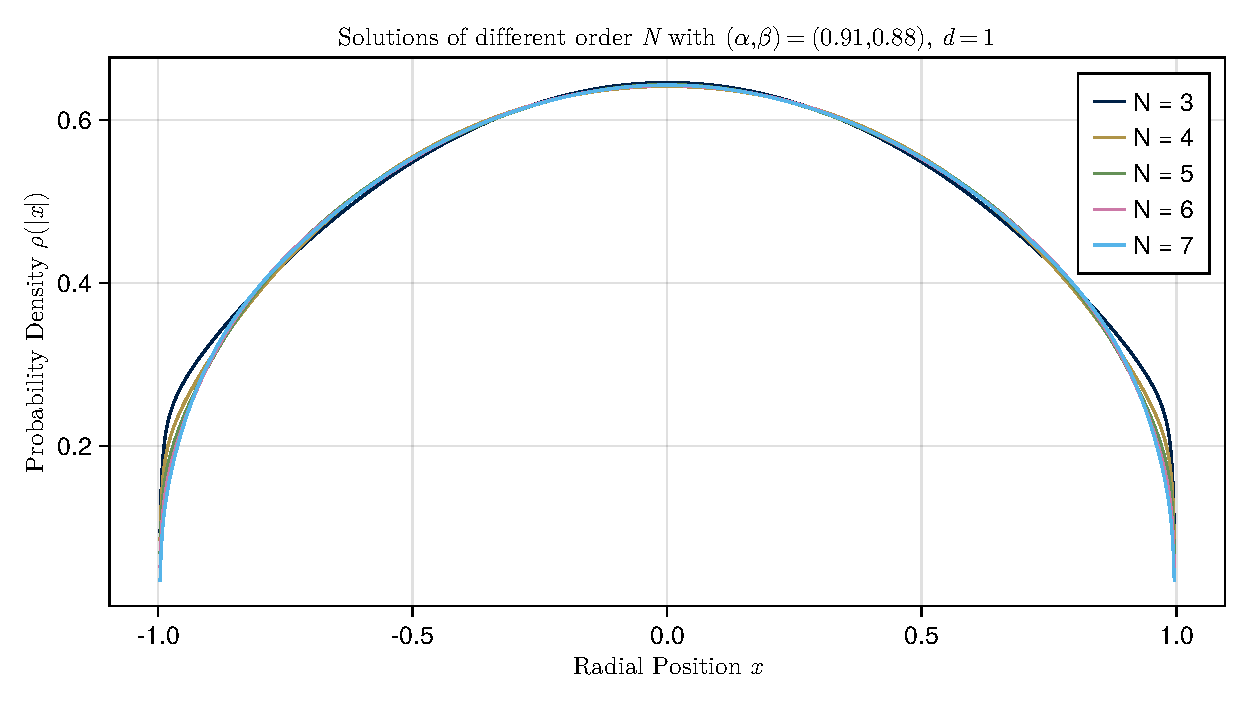
\includegraphics[width=0.8\linewidth]{results/attrep/solution-increasing-order.pdf}
  \caption[Solutions of increasing orders]{Particle density distribution function solutions $\rho$ of increasing order $N$ to the attractive-repulsive problem with interaction potential $K_{\alpha, \beta}(r)$, $\alpha = 2.5$ and $\beta = 1.2$. Reflected along the y-axis for better visibility of the domain.}
  \label{fig:solution-increasing-order}
\end{figure}

An overview of solutions for varying parameters in an attractive-repulsive setting can be found in \Cref{fig:varying-parameters}.

% Full Section:
\section{Outer Optimisation Routine}
The unconstrained outer optimisation over the scalar value $R \in \R^+$, the radius of our domain $B_R(\vec{0})$, is carried out using \href{https://github.com/JuliaNLSolvers/Optim.jl}{Optim.jl}'s implementation \parencite{2023-optim-jl} of the \gls{lbfgs} optimisation method \parencite{1989-lbfgs}, an extension of BFGS for low-memory usage, using an estimate for the gradient based on \gls{ad} techniques.

As part of a comparison between multiple optimisation approaches, \gls{lbfgs} outperformed the Nelder-Mead and Newton trust region methods for our case, converging extremely quickly within only 3 iterations, 10 function calls and 10 evaluations of the gradient.
While the downhill simplex method by \citeauthor{1965-nelder-mead} did not converge to the desired local minimum (cf. \Cref{fig:outer-optimisation}), the trust region method using Newton's method to solve a quadratic model for each subproblem \parencite{1982-trust-region} also converged in only 3 iterations with only 4 function, gradient and Hessian evaluations.
Again, the values of the gradient and Hessian (in the case of a one-dimensional optimisation, simply the first and second derivatives), are obtained using \glstext{ad}.

The \gls{lbfgs} method converged with $\norm{\nabla E(R)} \approx 10^{-11}$ while the Newton trust region method converged at $\norm{\nabla E(R)} \approx 10^{-9}$.
The entire optimisation routine with \gls{lbfgs}, including function and gradient evaluations (solving a $12 \times 12$ linear system), takes \SI{28 \pm 4}{\milli\second} on an Intel\textregistered \, i7-5600U CPU running at \SI{2.6}{\giga\hertz}.

\begin{figure}[H]
  \centering
  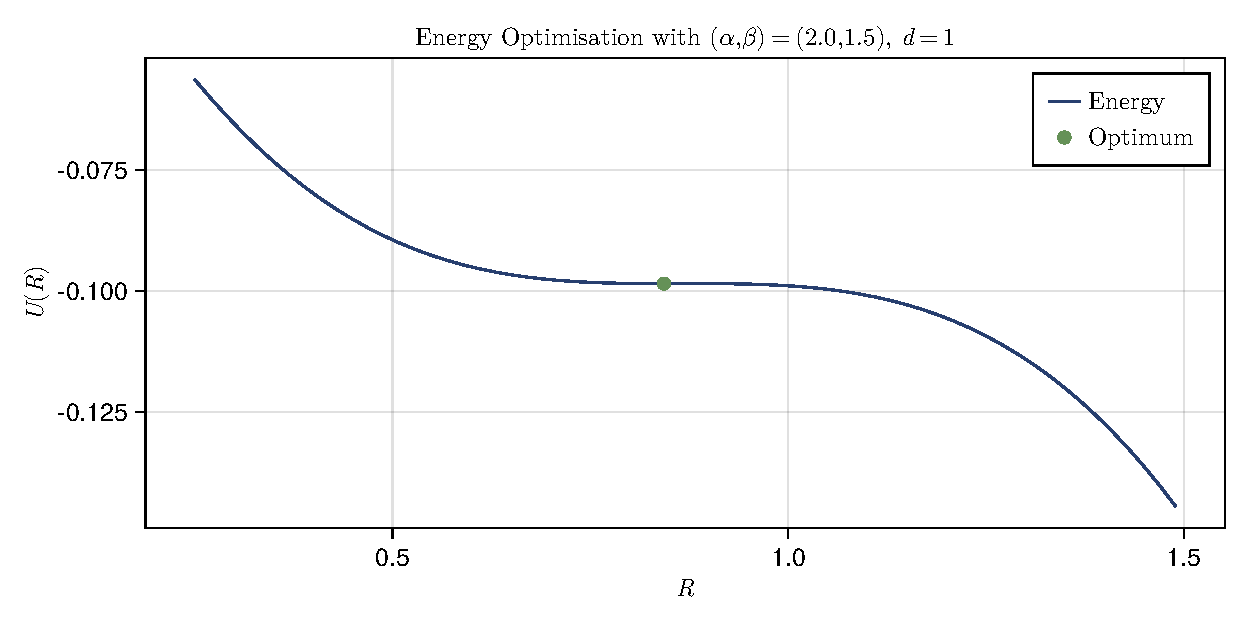
\includegraphics[width=0.8\linewidth]{results/known-analytic/outer-optimisation.pdf}
  \caption[Outer Optimisation Routine]{The total potential $U$ as a function of the support radius $R$. This is the goal function minimised by the outer optimisation routine.}
  \label{fig:outer-optimisation}
\end{figure}

Note that using this setup, the operators themselves do not need to be recomputed upon a change in $R$, cf. \Cref{eq:full-attrep-operator}.
The provided implementation uses \gls{lru} caching to automatically store operators for a given parameter set and order $N$.

\begin{lemma}{Unique Energy Minimum}{attrep-energy-min}
  Assuming an $N=1$ expansion of the density distribution $\rho$ according to \Cref{eq:ansatz} with $m \in \N_0$, for an attractive-repulsive interaction potential $K_{\alpha, \beta}(r) = \frac{r^\alpha}{\alpha} - \frac{r^\beta}{\beta}$, the energy minimum $E_{\rm min}$ is unique and given by
  $$E_{\rm min} = \left(\sfrac{I_{m,0}^{\alpha,\beta}}{I_{m,0}^{\alpha,\alpha}}\right)^\frac{1}{\alpha-\beta}\,,$$
  with $I_{m,n}^{\alpha,\alpha}$ as given in \Cref{thm:theorem216}.
\end{lemma}
\begin{proof}
  $$\frac{\partial E}{\partial R}$$
\end{proof}


\pagebreak
% Full Section:
\section{Comparison with Analytic Solutions}
As introduced in \Cref{sec:analytical-solutions}, there are some analytical solutions available which allow us to perform further analysis of the numerical method in these special cases.

The major advantage of a spectral method is its so-called \textit{spectral convergence}, sometimes also referred to as exponential convergence, cf. \Cref{def:spectral-convergence} from \cite{2023-damtp-spectral-methods}, verbatim.
\begin{definition}{Spectral Convergence}{spectral-convergence}
  An \(N\)-point approximation \(\varphi_N\) of a function f converges to \(f\) at spectral speed if \(|\varphi_N -f|\) decays pointwise in \([-1, 1]\) faster than \(\mathcal{O}(N^{-p})\) for any \(p = 1, 2, . . .\) so \(p \in \mathbb{N}\).
\end{definition}


For a given set of parameters with a known analytic solution (cf. \Cref{sec:analytical-solutions}), we compare growing orders of the spectral method's solution with the analytic expression in a set of 200 points and plot the pointwise error, cf. \Cref{fig:analytic-solution}.
The figure also shows how the outer optimisation routine approaches the optimal $R_{\rm opt}$ closer and closer for growing orders $N$.

\begin{figure}[H]
  \centering
  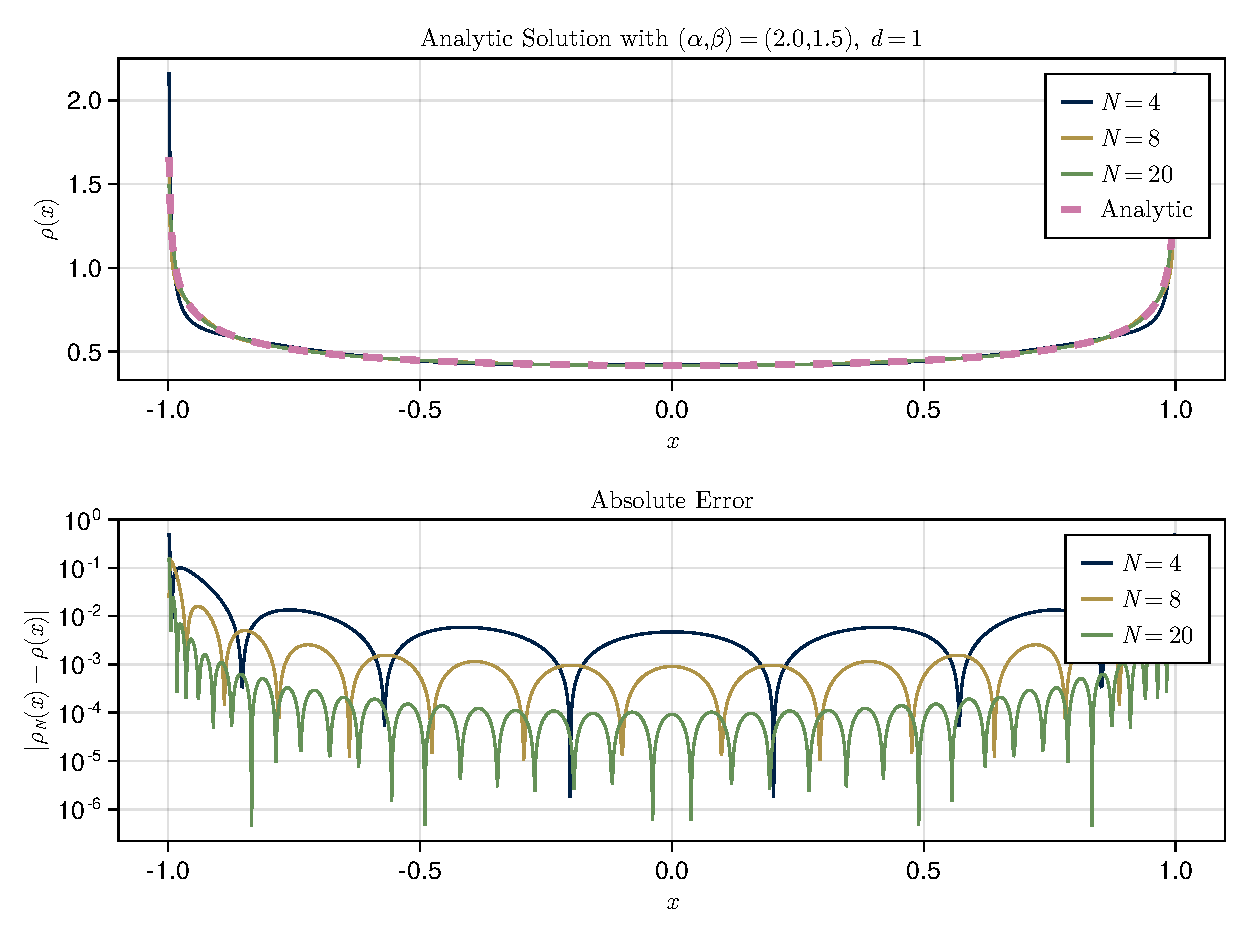
\includegraphics[width=\linewidth]{results/known-analytic/analytic-solution.pdf}
  \caption[Comparison with analytical solutions and error]{
    The analytic solution $\rho(x)$ given in \Cref{eq:analytical-solution-alpha-equal-2} compared to the (spectral method) solutions of different order $N$.
    The ``arches'' occur as a result of the roots of $\rho(x) - \rho_N(x)$, their number approximately equals the order $N$ (a polynomial of degree $N$ has at most $N$ roots).
  }
  \label{fig:analytic-solution}
\end{figure}

When choosing a specific parameter $a = \frac{1-\beta}{2}$, due to the choice of weighted basis in \Cref{eq:ansatz}, as compared to the form of the analytical solution in \Cref{eq:analytical-solution-alpha-equal-2}, convergence will be immediate after only one coefficient ($N=1$).
While this is excellent convergence behaviour, it is not very interesting for convergence analysis.
For this reason, we set $a = m - \frac{\alpha+d}{2}$ in the usual way and obtain convergence results in \Cref{fig:convergence-to-analytic}.
There are more analytic solutions available for other parameter ranges, which we will not analyse within the scope of this dissertation.

\begin{figure}[H]
  \centering
  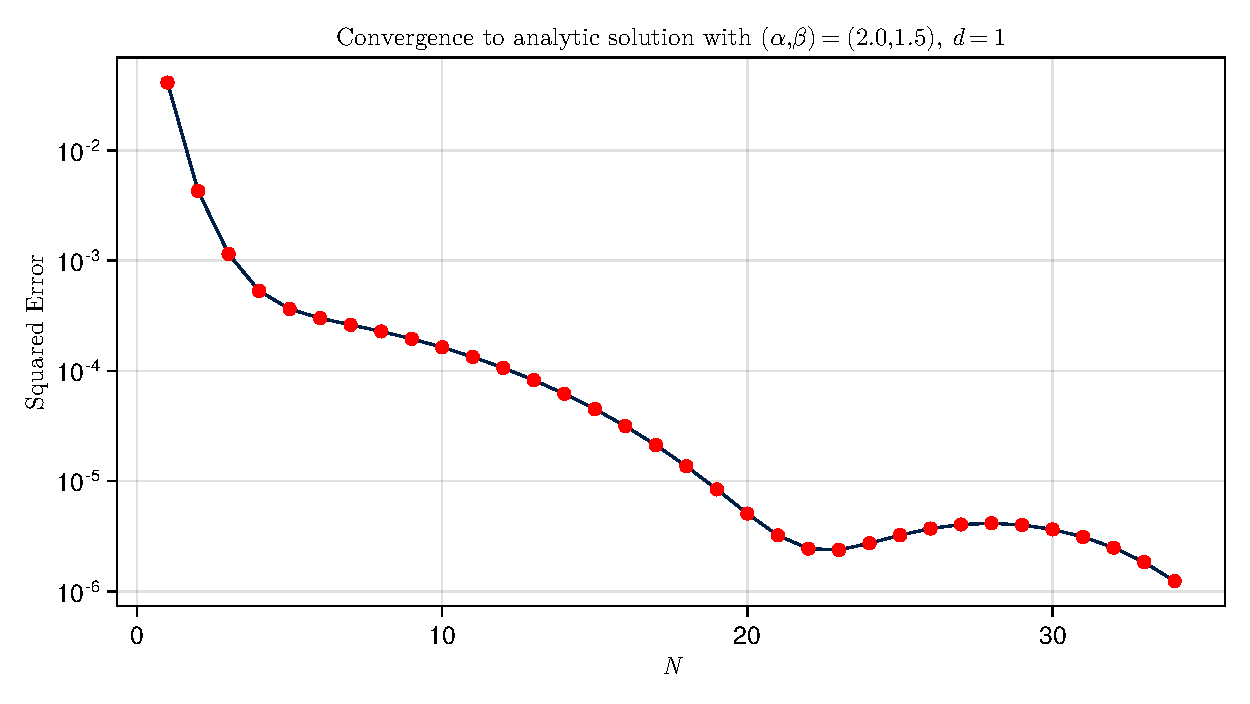
\includegraphics[width=0.8\linewidth]{results/known-analytic/convergence-to-analytic.pdf}
  \caption[Convergence to analytic solution]{Convergence of the numerical solution to the known analytic solution (cf. \Cref{eq:analytical-solution-alpha-equal-2}) in a special case where it is known, squared error plotted as a function of the highest order in the expansion $N$.}
  \label{fig:convergence-to-analytic}
\end{figure}


\section{Discussion}
For unknown analytic solutions, one can still perform a ``step-by-step'' convergence analysis, comparing the difference between two solutions of adjacent order for growing order $N$.
This does not always lead to clean improvements for every $N$, as can be seen in \Cref{fig:convergence}.

\begin{figure}[H]
  \centering
  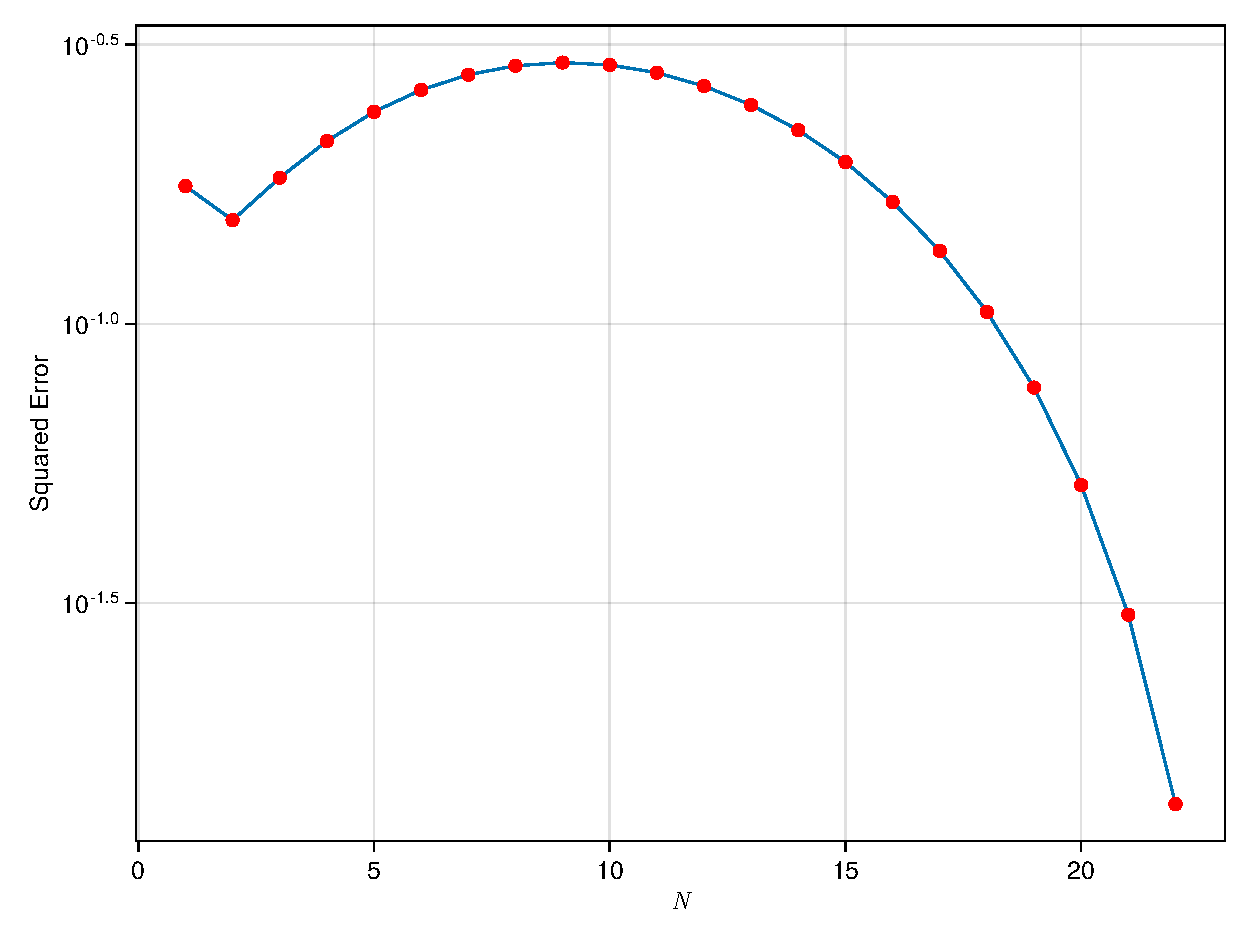
\includegraphics[width=0.8\linewidth]{results/attrep/convergence.pdf}
  \caption[Step-by-step convergence of solutions compared to order 24]{Step-by-step convergence of numerical solutions $\rho_N(x)$ as compared to $\rho_{24}(x)$, visualised using the squared error of the pointwise evaluation of both functions in $200$ points.}
  \label{fig:convergence}
\end{figure}
